% ---------------------------------------------------------------------------
% Section 5: Confirmation Study (M6; 540 runs on CPU)
% ---------------------------------------------------------------------------
\section{Confirmation Study}\label{sec:confirm}

The confirmation stage evaluates five preregistered arms (C-PM, B1-TCN,
B1-PM, B2-PM, LINEAR) plus one post-hoc addition (A-PM), each at 10
seeds on the 9 held-out flows
whose sources are source-blocked from the development set, with the frozen
teacher (T0) and the fixed-configuration PCA baseline as fixed references
(450 preregistered + 90 post-hoc = 540 student runs; all completed). The three preregistered comparisons are
evaluated at the source level ($n{=}9$ paired flows).

\begin{table}[t]
\centering
\caption{Confirmation-set VUS-PR (mean over 10 seeds) on 9 held-out
sources. The three preregistered pairwise comparisons are all
statistically non-significant at the source level (Section~\ref{sec:confirm-comparisons});
directional consistency with the development set is
noted in the text. Bold marks the row maximum (references included).}
\label{tab:confirm}
\scriptsize
\setlength{\tabcolsep}{3pt}
\begin{tabular}{lcccccccc}
\toprule
Flow & A-PM & C-PM & B1-TCN & B1-PM & B2-PM & LINEAR & T0 & PCA \\
\midrule
WADI (C1)            & 0.048 & 0.051 & 0.041 & 0.062 & 0.064 & 0.061 & 0.052 & \textbf{0.315} \\
Genesis (C2)         & 0.170 & 0.147 & 0.135 & 0.135 & 0.135 & 0.132 & 0.169 & \textbf{0.959} \\
Daphnet (C3)         & 0.307 & 0.317 & 0.231 & 0.245 & 0.245 & 0.252 & \textbf{0.416} & 0.111 \\
MGAB (C4)            & 0.009 & 0.008 & \textbf{0.124} & 0.011 & 0.010 & 0.016 & 0.009 & 0.009 \\
Yahoo (C5)           & 0.164 & 0.386 & 0.337 & \textbf{0.773} & 0.749 & 0.754 & 0.301 & 0.242 \\
IOPS (C6)            & 0.089 & 0.217 & 0.501 & 0.392 & 0.286 & \textbf{0.574} & 0.261 & 0.019 \\
MITDB (C7)           & 0.008 & 0.008 & \textbf{0.023} & 0.006 & 0.006 & 0.006 & 0.008 & 0.014 \\
NEweather (C8)       & 0.930 & 0.933 & 0.930 & 0.928 & 0.927 & 0.927 & 0.946 & \textbf{0.952} \\
AdExchange (C9)      & 0.182 & 0.185 & 0.177 & 0.183 & 0.181 & 0.183 & \textbf{0.227} & \textbf{0.227} \\
\midrule
Macro mean           & 0.212 & 0.250 & 0.278 & 0.304 & 0.289 & \textbf{0.323} & 0.265 & 0.316 \\
\bottomrule
\end{tabular}
\end{table}

\begin{table}[t]
\centering
\caption{Confirmation-set macro VUS-PR over nine held-out sources.
Mean with flow-level bootstrap 95\% CI (5{,}000 resamples) and median.
The three classical baselines are zero-tuning methods added under R11;
LOF-window is fit on the full unlabeled test segment (transductive,
non-streaming) and is excluded from streaming-deployment claims;
all other rows are preregistered arms, the teacher, or the fixed PCA
baseline.}
\label{tab:confirmci}
\scriptsize
\begin{tabular}{lccc}
\toprule
Detector & Macro mean & 95\% CI & Median \\
\midrule
Frozen teacher (T0) & 0.2654 & [0.114, 0.459] & 0.2269 \\
Robust-Z (zero tuning) & 0.2392 & [0.092, 0.443] & 0.1258 \\
MA-residual (zero tuning) & 0.3248 & [0.146, 0.525] & 0.2232 \\
LOF-window (zero tuning) & 0.3271 & [0.197, 0.500] & 0.2402 \\
PCA (fixed) & 0.3165 & [0.106, 0.561] & 0.2269 \\
Linear floor & 0.3229 & [0.124, 0.545] & 0.1835 \\
B1-PM (self-sup.) & 0.3039 & [0.113, 0.525] & 0.1835 \\
B1-TCN (self-sup.) & 0.2778 & [0.125, 0.473] & 0.1770 \\
B2-PM (forecast-dist.) & 0.2893 & [0.102, 0.509] & 0.1809 \\
C-PM (ranking-dist.) & 0.2501 & [0.102, 0.447] & 0.1846 \\
A-PM (score-dist.) & 0.2116 & [0.075, 0.406] & 0.1640 \\
\bottomrule
\end{tabular}
\end{table}

\begin{figure}[t]
\centering
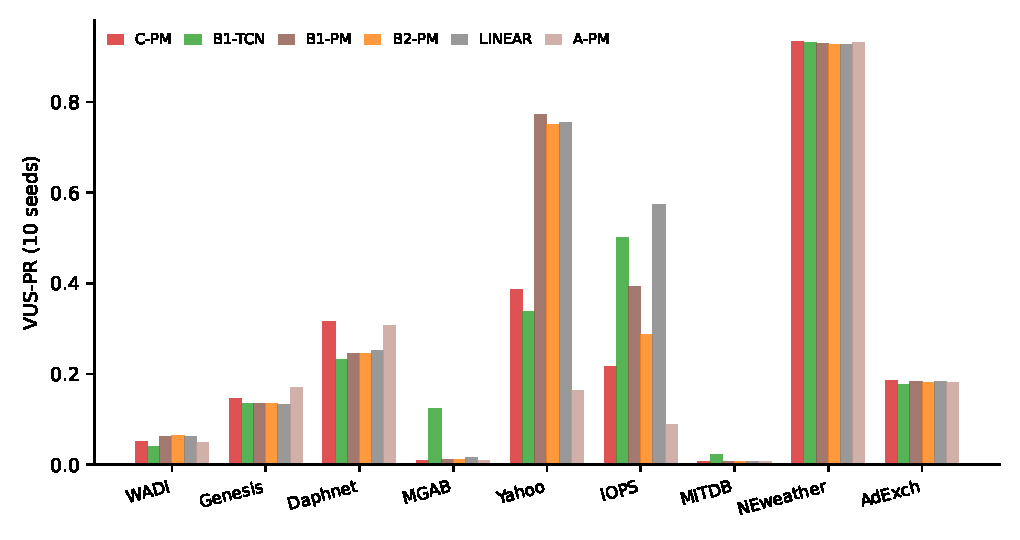
\includegraphics[width=0.9\textwidth]{figures/fig_exclusion_sensitivity.pdf}
\caption{Confirmation stage, per flow: VUS-PR (mean over 10 seeds) for
the five preregistered student arms plus the post-hoc A-PM addition on
the nine held-out sources (the same means as
Table~\ref{tab:confirm}, which additionally appends the teacher and
PCA references). No arm dominates across sources. The best
arm changes from source to source; the macro ordering of the student
arms is unchanged when
the shared-lineage WADI source or the confirmation NAB stream is
excluded.}
\label{fig:confirmflows}
\end{figure}

\subsection{Preregistered Comparisons}\label{sec:confirm-comparisons}
All three preregistered pairwise comparisons are statistically
non-significant at the source level ($n{=}9$; exact two-sided
Wilcoxon signed-rank; the exact test's minimum attainable two-sided
$p$ at $n{=}9$ is 0.0039, which bounds all reported $p$-values from
below). We report raw $p$ first and Holm-adjusted $p$ across the
three-comparison family in brackets. \textbf{B1-TCN vs.\ C-PM}:
mean difference $+0.028$ (bootstrap 95\%~CI $[-0.031,+0.103]$),
$p{=}1.0$ [Holm 1.0], matched-pairs rank-biserial $r{=}-0.02$
(3 wins / 6 losses); the positive mean is driven by a
single source (IOPS, $+0.28$) while C-PM wins pairwise on 6 of 9
sources. \textbf{LINEAR vs.\ C-PM}: $+0.073$
(CI $[-0.014,+0.195]$), $p{=}0.73$ [Holm 1.0], $r{=}+0.16$
(4 wins / 5 losses). \textbf{B2-PM vs.\ B1-PM}: $-0.015$
(CI $[-0.039,+0.000]$), $p{=}0.20$ [Holm 0.60], $r{=}-0.49$
(3 wins / 5 losses / 1 tie): replacing the
self-supervised target by the teacher's forecast provides no detectable
benefit and trends harmful, whereas on the development set the same
macro comparison favored B2-PM by $+0.027$ (0.244 vs.\ 0.217), so the
direction of this (non-significant) contrast is stage-dependent.
A fourth, post-hoc comparison (A-PM vs.\ C-PM: the score vs.\ ranking
interface; exploratory, excluded from the Holm family) is directionally
consistent with the development set
($-0.039$, CI $[-0.097,+0.003]$, $p{=}0.105$, rank-biserial
$-0.62$): the score arm is the weakest of the six student arms in the
confirmation set and the ranking arm the weakest of the five
preregistered ones, completing the score-to-ranking-to-self-supervision
ordering on held-out sources.
Under the preregistered 0.05 VUS-PR margin, the
B2-PM vs.\ B1-PM 95\% CI lies entirely within $\pm0.05$, so
equivalence of the two \emph{training targets} at the mean-source
level is supportable under an interval-based TOST reading (the more
conservative 95\% two-sided CI used here implies the 90\% TOST
criterion is met; $\Delta$ is the mean over the nine sources of the
per-source VUS-PR difference, CIs by source-level bootstrap); the
intervals for
B1-TCN vs.\ C-PM and LINEAR vs.\ C-PM extend to $+0.10$ and $+0.19$
respectively, so the study is underpowered to rule out differences of
that size. Table~\ref{tab:confirmci} consolidates the confirmation-set macro
comparison with flow-level bootstrap intervals, medians, and the three
zero-tuning classical baselines added under revision R11.
The classical additions sharpen the headline.
LOF-window (0.327) and MA-residual (0.325) land above every neural
arm and the fixed PCA baseline, and the frozen teacher itself (0.265)
falls below two zero-tuning methods.
The teacher-distilled arms (C-PM 0.250, A-PM 0.212) close the table's
lower half, so the boundary verdict gains a classical anchor: within
the tested configurations, no teacher signal we can measure survives
transfer as a quality advantage over zero-tuning classical scorers.
As a reference point for statistical power, with $n{=}9$ paired
sources, $\alpha{=}0.05$ two-sided, and 80\% power, the minimum
detectable effect is approximately $0.93\,\sigma_d$ of the paired
differences, about $0.10$ VUS-PR for the observed B1-TCN spread
($\sigma_d{\approx}0.10$) and about $0.15$ for the LINEAR spread
($\sigma_d{\approx}0.16$), matching the upper range the two favorable
CIs allow.

\subsection{Directional Consistency and Practical Reading}\label{sec:confirm-reading}
Although none of the differences is significant on nine sources, the
directional pattern replicates the development set. The two arms that do
not use the teacher's scores, namely LINEAR and B1-PM, have the two highest macro means among the student arms (PCA, a reference, is 0.316)
(macro 0.323 and 0.304 vs.\ 0.250 for the best score-distilled arm), the
forecast-distilled arm sits between (0.289), the score arm A-PM is the
weakest of the six student arms (0.212), and the exploration-stage
champion C-PM is the weakest of the five preregistered arms.
Two sources illustrate the conditional structure. On Yahoo the
self-supervised students dominate everything (B1-PM 0.773 vs.\ teacher
0.301 and C-PM 0.386), whereas on WADI and Genesis the PCA baseline
dominates everything (0.315 and 0.959 vs.\ $\le$0.064 and $\le$0.170
for every other method).
On NEweather every method exceeds 0.92. Exclusion sensitivity. Dropping
the WADI source (iTrust lineage shared with dev SWaT) or the
confirmation NAB stream leaves the arm ordering unchanged (e.g., macro
LINEAR/B1-PM/C-PM = 0.323/0.304/0.250 full, 0.356/0.334/0.275 without
WADI, 0.340/0.319/0.258 without NAB), so neither shared-lineage caveat
drives the directional pattern.
A stratified re-analysis (R10) reinforces this reading.
The confirmation set contains no dead flow on which every method falls
below 0.02 VUS-PR, so the macro comparison is not diluted by
unsignalable sources.
In the four teacher-null flows the strongest teacher-free arms widen
their lead (LINEAR 0.351 versus C-PM 0.165 mean).
In the five sources where the teacher matches or beats the best
self-supervised arm per flow (Genesis, Daphnet, MITDB, NEweather,
NAB-adexchange), score distillation adds only $+0.018$ mean VUS-PR over
that arm, while the fixed PCA baseline still dominates that subgroup
(0.453).
A prospective extension (revision R16) adds one fully independent
tenth source (CATSv2, 153{,}173 test points, 5{,}900 anomalies).
On this source every arm collapses to low absolute levels (0.036 to
0.077), score distillation shows a small edge over self-supervision
(0.077 versus 0.036), and the zero-tuning LOF-window scorer dominates
the source at 0.246.
The primary-set ordering is unchanged on the pooled ten-source sample,
and the boundary verdict gains a classical anchor on new ground.
The neural arms retain one exploratory niche.
On the 66-channel SWaT development source the best self-supervised
student (0.568) exceeds the strongest classical baseline there (PCA at
0.446), an observation we do not extrapolate beyond this source.
Figure~\ref{fig:confirmflows} shows the
per-flow results behind this analysis. The honest summary is twofold:
(i)~\emph{no arm is significantly better than any other at this sample
size}. The study cannot rule out differences of the size the intervals
allow (up to $+0.10$ for B1-TCN vs.\\ C-PM and $+0.19$ for LINEAR
vs.\\ C-PM); and (ii)~across both stages, 29 preregistered flows from 22
original data collections, and 1{,}270 preregistered primary-grid runs
(1{,}856 total including all disclosed controls and additions),
\emph{we find no evidence that a frozen TSFM teacher, through either a
score or a forecast interface, improves a lightweight edge detector
over self-supervised or even linear training under the same budget},
while the fidelity analysis (Section~\ref{sec:dev-fidelity}) shows the
score interface does not even transfer the teacher's ranking behavior.

\subsection{Cost Axis}\label{sec:confirm-cost}

\begin{figure}[t]
\centering
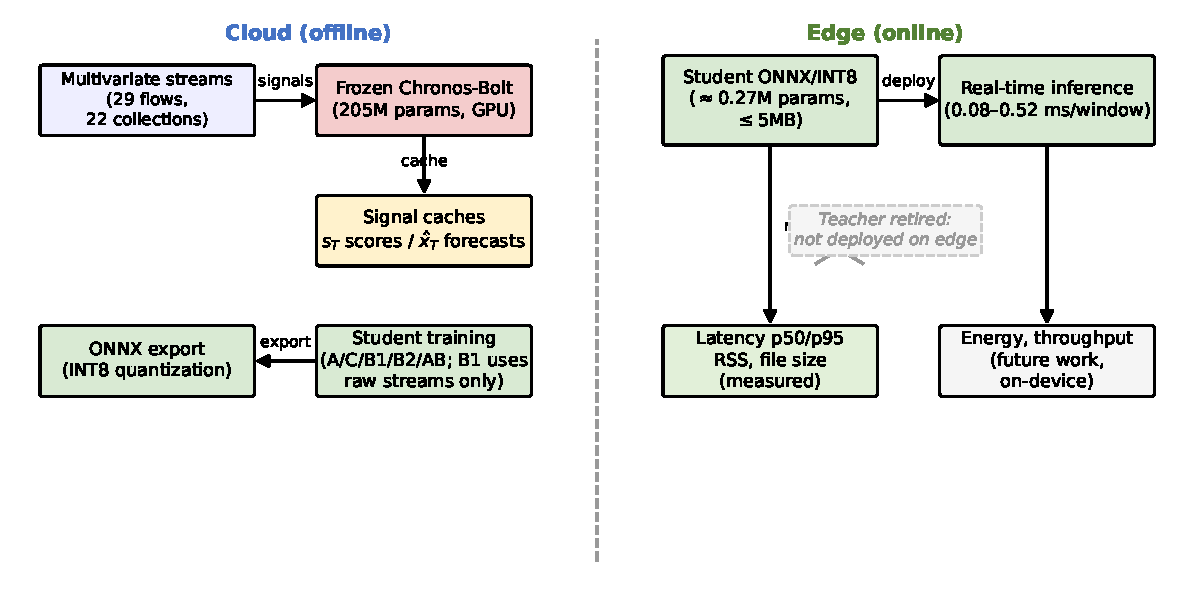
\includegraphics[width=0.95\textwidth]{figures/fig_deployment.pdf}
\caption{Deployment split. All teacher-dependent computation, namely scoring
the training segments and caching its score and forecast
signals, runs offline
in the cloud stage (arm B1 trains on the raw streams alone); the
teacher is retired before deployment. The edge
stage runs the exported student artifact alone ($\approx$0.27M
parameters, ONNX, optional INT8)
and reports the measured quantities of this section (per-window
latency, file size, peak RSS), on the desktop and now also on a
Raspberry~Pi~4B at the reference dimension, including a ten-minute
sustained-throughput check; energy profiling remains future work.}
\label{fig:deployment}
\end{figure}

Two budget tiers anchor the cost axis.
Tier E1 requires a per-window p95 latency below 1\,ms and an
artifact of at most 1\,MB; tier E2 extends both to 5\,ms and
5\,MB.
Thresholds are defined on desktop single-thread measurements; the
Raspberry~Pi~4B figures are device-side validation, not tier
definitions.
The computational budget of the full study is modest.
Building the Chronos-Bolt teacher cache over all thirty flows (twenty-nine
preregistered plus the R16 extension) took 17.4
GPU-hours (mean 35 minutes per flow), a one-time cost shared by every
distilled arm.
Each student training run completes in 1--12 minutes on a single GPU
(mean 84 seconds over the 450 confirmation runs, 12.5 GPU-hours in
total), and the complete 1{,}856-run study fits within roughly 40
GPU-hours of student training plus the cached teacher passes.
All cost figures below are measured on \emph{trained} artifacts
(case-C students retrained once per architecture--dimension
configuration under the confirmation-stage recipe, exported to ONNX,
and re-timed on an idle machine. Appendix~\ref{app:cost} reports the
full matrix with round-to-round ranges). On the desktop CPU
(single-thread ONNX Runtime, batch 1), the
linear floor requires 0.009--0.049\,ms p95 with files at or below
0.13\,MB (budget tier E1 at every dimension). PatchMLP-lite runs in
0.092--0.194\,ms FP32 and, after dynamic INT8 quantization,
0.058--0.116\,ms with 0.22--0.47\,MB files, inside E1 at every tested
dimension (1 to 248 channels). TCN-lite runs in
0.414--0.653\,ms FP32 (E1 at low channel counts by latency; its file
crosses 1\,MB from 66 channels, so E2 there), but its dynamically
quantized variant is 10.3--12.2$\times$ \emph{slower} (quantized
convolution kernels in the runtime), so INT8 is recommended for the
MLP-mixer architecture only. Quantization also perturbs quality. The
INT8-minus-FP32 VUS-PR drift of the exported artifacts is within
$\pm$0.01 on most configurations and even reaches $+0.074$ and $+0.097$
on the 66- and 248-channel PatchMLP students (quantization noise as
regularization), with one loss of $-0.066$ on the 66-channel linear
floor (Appendix~\ref{app:cost}); the linear floor, at most 0.13\,MB,
has no need to quantize.

The frozen teacher (Chronos-Bolt-base) is in a different cost class
entirely. Figure~\ref{fig:deployment} places teacher and student on
opposite sides of the deployment boundary. Its offline scoring pass
over the training segments of all 29 flows cost 15.4 GPU-hours (mean
32 minutes per flow), a one-time cost amortized across every student
trained from the cache, but non-trivial for a single deployment and
zero for self-supervised students. Measured on the same idle machine
(12th-Gen Intel Core
i7-12700F, ONNX Runtime 1.28, PyTorch 2.13; single CPU thread) under
two matching protocols, scoring one point costs 64.7\,ms at batch 64
and 122.9\,ms at batch 1 (the deployment-faithful setting; 512-point
context, end-to-end including normalization and aggregation). The
students' end-to-end cost over full test splits (stride-1 windows,
trained artifacts, two development flows and one held-out
confirmation flow) is 0.07--0.51\,ms p50 per window (p95 up to
0.62\,ms): roughly
\emph{200--1500$\times$} faster than the teacher
at batch 1, depending on architecture and channel count. Combined with
the quality results (Figure~\ref{fig:cost}), the cost axis completes the picture. The teacher is
simultaneously slower than every student by orders of magnitude and not
better than the strongest of them on held-out sources. Peak RSS is
process-level. For the sub-million-parameter students the in-process
delta is below measurement noise ($\le$6\,MB over the ORT runtime
baseline), and cold-start is excluded from the per-window figures (both
disclosed). The Raspberry~Pi~4B on-device measurements follow the identical
protocol (single-thread ONNX Runtime, batch 1, $L=128$, CPU governor
pinned to performance).
On the board, the linear floor measures 0.44\,ms p95, the quantized
PatchMLP student 2.00\,ms, and the TCN student 15.47\,ms at the
66-channel reference.
Process peak RSS stays at 59--62\,MB with no thermal throttling
(49--52$^\circ$C).
These board figures sit 25--33$\times$ above the matching desktop
medians.
The linear floor and the quantized PatchMLP student stay inside their
E1 and E2 budget tiers on the board, while the FP32 TCN student lands
above E2, reinforcing the recommendation to deploy the quantized
MLP-mixer student.
Even on the board, every student remains 8--278$\times$ cheaper than
the teacher's desktop batch-1 cost of 122.9\,ms.
The teacher itself is not deployable on the board at all: Chronos-Bolt-base
requires 2.4\,s per scored point on the same device (batch 1, context
512, end-to-end), roughly 19.5$\times$ its desktop cost and 155 to
5{,}428$\times$ above the student artifacts.
